\section{Architecture}
\label{sec:architecture}

Providing a state-of-the-art architecture and setup is one of the main goals of the new portfolio management game project. As a general direction, moving to a web-based application was defined early on as a replacement for the previous decentral solution.

\begin{figure}[h!]
  \centering
  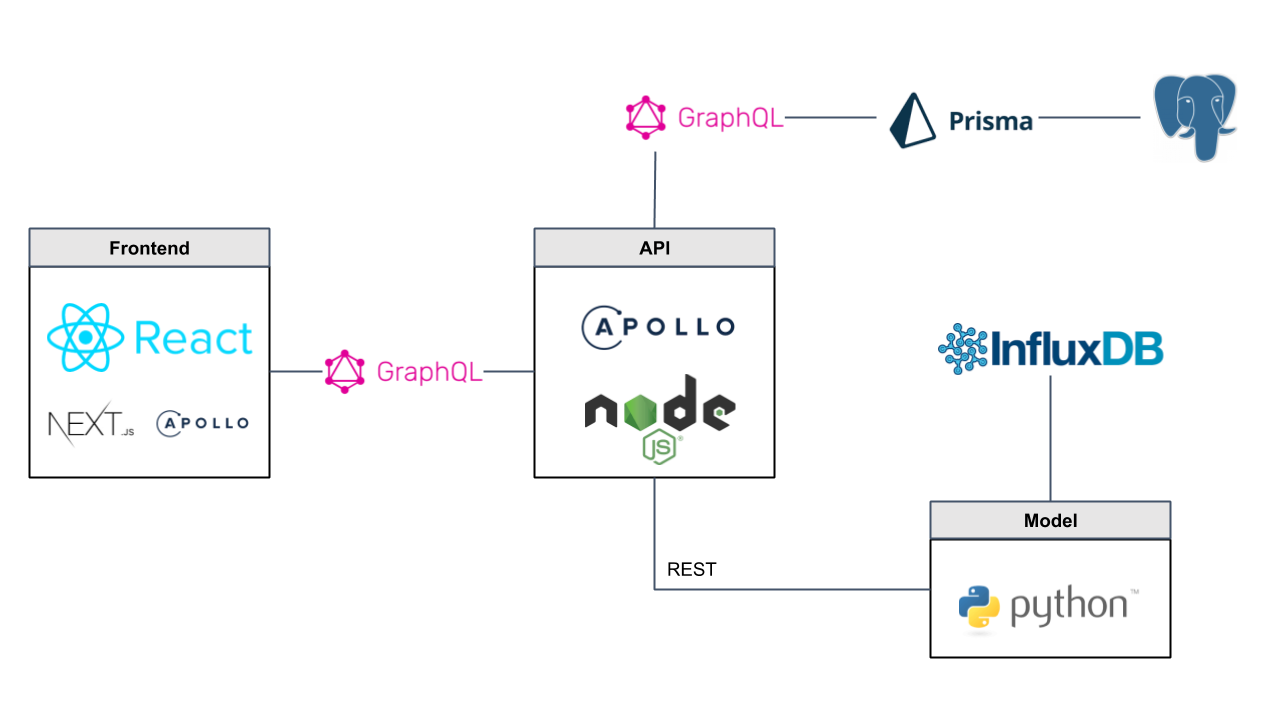
\includegraphics[scale=0.45]{img/architecture.png}
  \caption{PFM game architecture}
\end{figure}


\subsection{Frontend (pfm-react)}
\begin{flushright}
  \textbf{Repository:} https://git.ibf-devops.ch/wb/pfm-game/pfm-react
\end{flushright}

The application frontend is structured as a single-page application for use in web browsers optimized especially for Google Chrome. Contrary to the native Windows application of the old game, this allows for effortless setup and resolves many problems with manual data transfer (either via USB for game data or on paper for reporting). The single-page app paradigm has become more and more popular with frameworks like React, Angular, and Vue being used by millions of developers. As such, our implementation of the game is based on the latest versions of the ReactJS and NextJS framework.\footnote{See https://reactjs.org/ and https://nextjs.org/}


\subsection{GraphQL}

Traditional web applications have been using the RESTful paradigm for a long time. In a RESTful application, different types of entities are accessible on different endpoints and using different methods. For example, a GET request on a /customers endpoint could return a list of all customers.\\

Contrary to this, GraphQL is a new way of fetching data in a declarative fashion. The project has been initially developed at Facebook, was open-sourced in 2015, and has become widely used since that time. The key concept, declarative data fetching, can be summarized as an API response having the same structure as the corresponding request. Additionally, all communication using GraphQL is bound to a single endpoint, as the response depends solely on the content of the request. \footnote{See https://graphql.org/}\\

If we wanted to request a list of users from our GraphQL API, we could make an exemplary request as can be seen in listing~\ref{lst:graphql_request}. The corresponding example response is shown in listing~\ref{lst:graphql_response}.

\begin{multicols}{2}
  \vspace*{\fill}
  \begin{lstlisting}[caption=GraphQL request, label=lst:graphql_request]
query {
  users {
    id
    email
    username
  }
}
  \end{lstlisting}
  \columnbreak
  \begin{lstlisting}[caption=GraphQL response, label=lst:graphql_response]
{
  users [{
      email: "rolandschlaefli@gmail.com",
      username: "roland"
    },
    {
      email: "pascal_zehnder@outlook.com",
      username: "pascal"
  }]
}
  \end{lstlisting}
\end{multicols}

This new approach to data fetching allows us to fetch data directly where it is needed. For example, specific details regarding a user might be fetched only when a form is shown to edit these data. Furthermore, as requests using GraphQL only contain the fields that were actually requested (and not every field available), the data fetching consumes fewer resources and therefore fetches data within a shorter timeframe.


\subsection{API (pfm-api)}
\begin{flushright}
  \textbf{Repository:} https://git.ibf-devops.ch/wb/pfm-game/pfm-api
\end{flushright}

Any application wanting to consume API data using GraphQL needs a special endpoint that supports this format. As such, our application backend has to support GraphQL as its main communication language. There are some popular server-side frameworks for this case, including an official reference implementation maintained by Facebook. A combination of a NodeJS server integrated with the Apollo Server framework serves as a good basis for our GraphQL endpoint.\footnote{See https://nodejs.org/en/ and https://www.apollographql.com/docs/apollo-server/}\\

The core responsibilities of the API are handling the authentication and authorization of requests, structuring the main business logic into services (such as account-, game-, model-, play- and scoring-service), handling all communications with the market model, as well as managing the Prisma database access layer for data persistence.


\subsection{Prisma}

\begin{flushright}
  \textbf{Repository:} https://git.ibf-devops.ch/wb/pfm-game/pfm-api
\end{flushright}

The Prisma database access layer is a middleware that sits in between the API and a Postgres database. The Prisma instance provides a single GraphQL endpoint with which database entities can be created, deleted, updated, or read. Additionally, Prisma handles everything related to database management, including schema creation, migrations, and maintenance. The underlying database schema is defined using a GraphQL schema language, using which types and relations can be modeled.\footnote{See https://www.prisma.io/}


\subsection{Model (pfm-model)}

\begin{flushright}
  \textbf{Repository:} https://git.ibf-devops.ch/wb/pfm-game/pfm-model
\end{flushright}

While the API provides services for all the persistence and input related logic, the model is responsible for everything related to the actual calculations and computations for the game. This includes everything from extracting available assets from the InfluxDB time-series database to scoring teams based on many input parameters.\\

The model is structured into several Python modules that can be accessed by the API using specialized REST endpoints. The model is not connected to the main application database and performs all of its calculations in a stateless manner (except that it fetches historical asset data from the specialized InfluxDB instance). This allows for keeping the API logic at a bare minimum, moving most of the logic into the modules.\footnote{See https://falconframework.org/}


\subsection{Simulation (pfm-model)}

\begin{flushright}
  \textbf{Repository:} https://git.ibf-devops.ch/wb/pfm-game/pfm-model
\end{flushright}

The portfolio management simulation is a project that was taken on during the course of a Master thesis at the Department of Banking and Finance. Even though the simulation was executed as a separate project, the project goals are tightly coupled: the results of the simulation project are planned to be integrated into the game application in the near future.\\

With said integration, it would be possible to pseudo-randomly generate new asset time-series with which a game could be played, instead of basing the entire game on historical data. By tuning some parameters, game masters could then influence the generation of said time-series to e.g. simulate a period of recession.\\

The simulation project is structured as a collection of Python modules that incrementally build from raw asset data, over sector portfolio generation, and up to simulated asset time-series. Due to the coupling of the project, we provided support for the deployment and infrastructure setup and developed a Python REST API for the project. Additionally, some parts of the InfluxDB data hydration scripts had to be reimplemented due to inefficiencies and incompatibilities.\\

Further details are described in the thesis related to the simulation project. As such, we do not describe any further details here.


\subsection{Continuous Integration}

To support development efforts over the course of the pfm-game project, a key factor has been the setup of a successful continuous integration (CI) pipeline at the beginning of the project. Due to previous positive experiences with CI and other DevOps paradigms, we decided that each subproject should be continuously integrated and published as a Docker container.
